% Options for packages loaded elsewhere
\PassOptionsToPackage{unicode}{hyperref}
\PassOptionsToPackage{hyphens}{url}
%
\documentclass[
  10pt,
]{article}
\usepackage{amsmath,amssymb}
\usepackage{iftex}
\ifPDFTeX
  \usepackage[T1]{fontenc}
  \usepackage[utf8]{inputenc}
  \usepackage{textcomp} % provide euro and other symbols
\else % if luatex or xetex
  \usepackage{unicode-math} % this also loads fontspec
  \defaultfontfeatures{Scale=MatchLowercase}
  \defaultfontfeatures[\rmfamily]{Ligatures=TeX,Scale=1}
\fi
\usepackage{lmodern}
\ifPDFTeX\else
  % xetex/luatex font selection
\fi
% Use upquote if available, for straight quotes in verbatim environments
\IfFileExists{upquote.sty}{\usepackage{upquote}}{}
\IfFileExists{microtype.sty}{% use microtype if available
  \usepackage[]{microtype}
  \UseMicrotypeSet[protrusion]{basicmath} % disable protrusion for tt fonts
}{}
\makeatletter
\@ifundefined{KOMAClassName}{% if non-KOMA class
  \IfFileExists{parskip.sty}{%
    \usepackage{parskip}
  }{% else
    \setlength{\parindent}{0pt}
    \setlength{\parskip}{6pt plus 2pt minus 1pt}}
}{% if KOMA class
  \KOMAoptions{parskip=half}}
\makeatother
\usepackage{xcolor}
\usepackage[margin=21mm]{geometry}
\usepackage{longtable,booktabs,array}
\usepackage{calc} % for calculating minipage widths
% Correct order of tables after \paragraph or \subparagraph
\usepackage{etoolbox}
\makeatletter
\patchcmd\longtable{\par}{\if@noskipsec\mbox{}\fi\par}{}{}
\makeatother
% Allow footnotes in longtable head/foot
\IfFileExists{footnotehyper.sty}{\usepackage{footnotehyper}}{\usepackage{footnote}}
\makesavenoteenv{longtable}
\usepackage{graphicx}
\makeatletter
\def\maxwidth{\ifdim\Gin@nat@width>\linewidth\linewidth\else\Gin@nat@width\fi}
\def\maxheight{\ifdim\Gin@nat@height>\textheight\textheight\else\Gin@nat@height\fi}
\makeatother
% Scale images if necessary, so that they will not overflow the page
% margins by default, and it is still possible to overwrite the defaults
% using explicit options in \includegraphics[width, height, ...]{}
\setkeys{Gin}{width=\maxwidth,height=\maxheight,keepaspectratio}
% Set default figure placement to htbp
\makeatletter
\def\fps@figure{htbp}
\makeatother
\setlength{\emergencystretch}{3em} % prevent overfull lines
\providecommand{\tightlist}{%
  \setlength{\itemsep}{0pt}\setlength{\parskip}{0pt}}
\setcounter{secnumdepth}{5}
\ifLuaTeX
  \usepackage{selnolig}  % disable illegal ligatures
\fi
\usepackage{bookmark}
\IfFileExists{xurl.sty}{\usepackage{xurl}}{} % add URL line breaks if available
\urlstyle{same}
\hypersetup{
  pdftitle={State-Selected Reheating in Exact Z6 Chronometry},
  pdfauthor={Technical research note v0.9},
  hidelinks,
  pdfcreator={LaTeX via pandoc}}

\title{State-Selected Reheating in Exact Z6 Chronometry}
\usepackage{etoolbox}
\makeatletter
\providecommand{\subtitle}[1]{% add subtitle to \maketitle
  \apptocmd{\@title}{\par {\large #1 \par}}{}{}
}
\makeatother
\subtitle{An orbit-symmetric reheaton, transient vacuum selection,
defect control, and the primordial perturbation spectrum}
\author{Technical research note v0.9}
\date{17 August 2026}

\begin{document}
\maketitle

{
\setcounter{tocdepth}{3}
\tableofcontents
}
\section{Executive result}\label{executive-result}

An explicit reheating model can produce

\[
\xi_0=1,
\qquad
\xi_5=0.25,
\qquad
\xi_{1,2,3,4}\ll1,
\]

without inserting a sector-dependent constant into the microscopic
Lagrangian. The essential distinction is

\[
\boxed{
\text{the action remains exactly }Z_6\text{-symmetric, while the cosmological state is not.}
}
\]

This distinction is not cosmetic. A hard reheating spurion that couples
only to one replica generically feeds into the protected threshold
sector and generates a lower-harmonic zero-temperature potential. That
is precisely the radiative-stability obstruction identified in recent
replicated-sector analyses. The construction developed here avoids that
obstruction by using:

\begin{enumerate}
\def\labelenumi{\arabic{enumi}.}
\tightlist
\item
  two complete reheaton orbits, \(X_k\) and \(Y_k\), with exact cyclic
  couplings;
\item
  a transient one-hot selector state \(Q_0\neq0\), selected during
  inflation;
\item
  kinematic production of only one light reheaton eigenstate \(R_0\);
\item
  restoration of the selector to the unique symmetric vacuum before
  reheaton decay;
\item
  a fixed, orbit-symmetric nearest-neighbour mixing angle,
  \(\tan\theta=1/16\).
\end{enumerate}

The selected reheaton then decays as

\[
R_0\longrightarrow
\begin{cases}
\mathcal S_0,&B_0=256/257,\\
\mathcal S_5,&B_5=1/257,
\end{cases}
\]

and therefore

\[
\boxed{
\frac{T_5}{T_0}
=
\left(\frac{B_5}{B_0}\right)^{1/4}
=\frac14.
}
\]

The remaining four sectors have no tree-level reheaton channel. A
deliberately conservative estimate of gravity-only leakage gives

\[
\xi_{1,2,3,4}\lesssim4.7\times10^{-3}.
\]

For one complete adjacent Standard Model copy at \(\xi_5=0.25\),

\[
\boxed{
\Delta N_{\rm eff}=0.0289,
}
\]

below the present 95\% upper bound \(\Delta N_{\rm eff}<0.107\).

The model also predicts the perturbation spectrum rather than only the
homogeneous temperature history. A low-scale hilltop-hybrid benchmark
with

\[
H_*=10^8\ {\rm GeV}
\]

gives

\[
A_s=2.10\times10^{-9},
\qquad
n_s=0.9682,
\qquad
r=1.63\times10^{-13},
\]

and

\[
f_{\rm NL}^{\rm local}\simeq0.0133.
\]

Because both populated radiation sectors arise from one parent with
fixed branching fractions,

\[
\boxed{
\zeta_0=\zeta_5=\zeta,
\qquad
S_{50}=3(\zeta_5-\zeta_0)=0
}
\]

at linear order. The extra radiation is therefore adiabatic, not a
dark-radiation isocurvature mode.

The compact chronometric field remains a spectator during inflation. Its
initial fluctuation is

\[
\delta x_{\rm reh}
=
\frac{H_*}{2\pi f_a}
=6.54\times10^{-4},
\qquad
x\equiv a/f_a.
\]

Numerical evolution through the heavy-threshold thermal potential, the
QCD crossover and baryon locking gives

\[
\left|\frac{\delta x_{\rm rec}}{\delta x_{\rm reh}}\right|
=1.01\times10^{-6},
\]

so that

\[
\delta x_{\rm rec}=-6.62\times10^{-10}.
\]

The corresponding perturbation of the QCD lock is

\[
\boxed{
\left|\delta\ln\frac{\Lambda_{\rm QCD}}{\chi}\right|_{\rm rec}
=1.32\times10^{-23}.
}
\]

Thus the model produces the required background asymmetry while
predicting essentially pure adiabatic primordial perturbations.

The current verdict is:

\begin{longtable}[]{@{}lr@{}}
\toprule\noalign{}
Requirement & Verdict \\
\midrule\noalign{}
\endhead
\bottomrule\noalign{}
\endlastfoot
Exact microscopic \(Z_6\) & \textbf{PASS} \\
\(\xi_5=0.25\) & \textbf{PASS exactly} \\
Other replicas cold & \textbf{PASS perturbatively} \\
Hard-spurion radiative obstruction & \textbf{EVADED conditionally} \\
Selector and reheaton stability & \textbf{PASS at benchmark} \\
Domain walls in observable patch & \textbf{PASS conditionally} \\
Dark-radiation isocurvature & \textbf{ZERO at linear order} \\
Chronometric isocurvature & \textbf{NEGLIGIBLE numerically} \\
\(\Delta N_{\rm eff}\) & \textbf{PASS} \\
Full nonperturbative preheating & \textbf{OPEN} \\
Discrete-gauge UV completion & \textbf{OPEN} \\
\end{longtable}

\section{The obstruction that the model must
evade}\label{the-obstruction-that-the-model-must-evade}

A generic asymmetric reheating interaction has the form

\[
\mathcal L_{\rm hard}
\supset
-\kappa_0\sigma H_0^\dagger H_0,
\]

with no corresponding orbit of interactions in the other sectors. The
coefficient \(\kappa_0\) is then a genuine \(Z_6\)-breaking spurion.
Even if introduced only for reheating, loops communicate the spurion to
the replicated coloured threshold masses,

\[
M_k(a)
=
M\left[1-\epsilon\cos\left(\frac a{f_a}+\frac{2\pi k}{6}\right)\right],
\]

and generate a first-harmonic vacuum contribution of schematic size

\[
\delta V(a)
\sim
\epsilon_b\epsilon M^4
\cos\left(\frac a{f_a}-\delta\right).
\]

That term is parametrically larger than the protected \(O(\epsilon^6)\)
potential. Therefore ordinary selective reheating is not compatible with
the cyclic radiative cancellation unless the reheating sector is
extraordinarily sequestered.

Our construction does not add \(\kappa_0\). Every coupling appears in a
complete orbit. The only quantity that distinguishes sector 0 is a
transient field configuration selected by inflation. Once that
configuration relaxes to the symmetric origin, the zero-temperature
action and vacuum again contain no lower-harmonic spurion.

The logical structure is

\[
\boxed{
\begin{aligned}
\text{hard sector label in a coupling}
&\Rightarrow
\text{permanent vacuum spurion},\\
\text{sector label in a transient occupation state}
&\Rightarrow
\text{finite-density potential only}.
\end{aligned}
}
\]

This is the central model-building move.

\section{Exact cyclic field content}\label{exact-cyclic-field-content}

Let the replicated matter sectors be

\[
\mathcal S_k,
\qquad
k=0,\ldots,5,
\]

with all indices understood modulo six. The exact cyclic transformation
is

\[
\mathsf z:
\mathcal S_k\mapsto\mathcal S_{k+1}.
\]

Introduce two real reheaton orbits

\[
X_k,
\qquad
Y_k,
\]

and six complex selector fields

\[
Q_k.
\]

They transform as

\[
\mathsf z:
X_k\mapsto X_{k+1},
\qquad
Y_k\mapsto Y_{k+1},
\qquad
Q_k\mapsto Q_{k+1}.
\]

The renormalisable reheaton Lagrangian is

\[
\begin{aligned}
\mathcal L_R
={}&
\frac12\sum_k(\partial X_k)^2
+
\frac12\sum_k(\partial Y_k)^2
-
\frac12m_X^2\sum_kX_k^2
-
\frac12m_Y^2\sum_kY_k^2
\\
&+
\mu_{XY}^2\sum_kX_kY_{k-1}
-
\mu_H\sum_k
\left(
X_kH_k^\dagger H_k
+
Y_kH_k^\dagger H_k
\right).
\end{aligned}
\]

The oriented mixing \(X_kY_{k-1}\) preserves \(Z_6\) but not the
additional reflection that would enlarge the group to \(D_6\). That
chirality in replica space is deliberate: it lets the selected reheaton
feed one sector and its clockwise neighbour.

The displayed interaction contains no privileged value of \(k\). A
numerical tensor check under 1,000 random cyclic shifts gives a maximum
residual

\[
2.13\times10^{-14},
\]

consistent with floating-point roundoff.

\section{Reheaton mixing and the exact temperature
ratio}\label{reheaton-mixing-and-the-exact-temperature-ratio}

For each \(k\), work in the pair

\[
(X_k,Y_{k-1}).
\]

Its mass matrix is

\[
\mathcal M_R^2
=
\begin{pmatrix}
 m_X^2&-\mu_{XY}^2\\
 -\mu_{XY}^2&m_Y^2
\end{pmatrix}.
\]

Define

\[
\begin{pmatrix}
R_k\\S_k
\end{pmatrix}
=
\begin{pmatrix}
\cos\theta&\sin\theta\\
-\sin\theta&\cos\theta
\end{pmatrix}
\begin{pmatrix}
X_k\\Y_{k-1}
\end{pmatrix}.
\]

The benchmark takes

\[
\tan\theta=\frac1{16},
\qquad
m_R=10^9\ {\rm GeV},
\qquad
m_S=6\times10^9\ {\rm GeV}.
\]

The corresponding microscopic mass parameters are

\[
m_X=1.0659\times10^9\ {\rm GeV},
\]

\[
m_Y=5.9886\times10^9\ {\rm GeV},
\]

and

\[
\sqrt{\mu_{XY}^2}=1.4761\times10^9\ {\rm GeV}.
\]

Both eigenvalues are positive. A 50,000-point scan over nearby positive
masses and mixing angles found no negative eigenvalue and verified

\[
\frac{\sin^2\theta}{\cos^2\theta}=\tan^2\theta
\]

to numerical precision.

For the selected state \(R_0\),

\[
\mathcal L_{R_0}
\supset
-\mu_HR_0
\left(
\cos\theta H_0^\dagger H_0
+
\sin\theta H_5^\dagger H_5
\right).
\]

At \(m_R\gg m_H\), summing the four real components of each Higgs
doublet gives

\[
\Gamma_0
=
\frac{\mu_H^2\cos^2\theta}{8\pi m_R},
\qquad
\Gamma_5
=
\frac{\mu_H^2\sin^2\theta}{8\pi m_R}.
\]

Consequently,

\[
\frac{\Gamma_5}{\Gamma_0}
=
\tan^2\theta
=
\frac1{256}.
\]

The total branching fractions are

\[
B_0=\frac{256}{257}=0.99610895,
\]

\[
B_5=\frac1{257}=0.00389105.
\]

For equal relativistic degrees of freedom at decay,

\[
\frac{T_5}{T_0}
=
\left(\frac{\rho_5}{\rho_0}\right)^{1/4}
=
\left(\frac{B_5}{B_0}\right)^{1/4}
=
\boxed{\frac14}.
\]

This is not a numerical fit. It is an exact algebraic consequence of the
mixing angle.

\begin{figure}
\centering
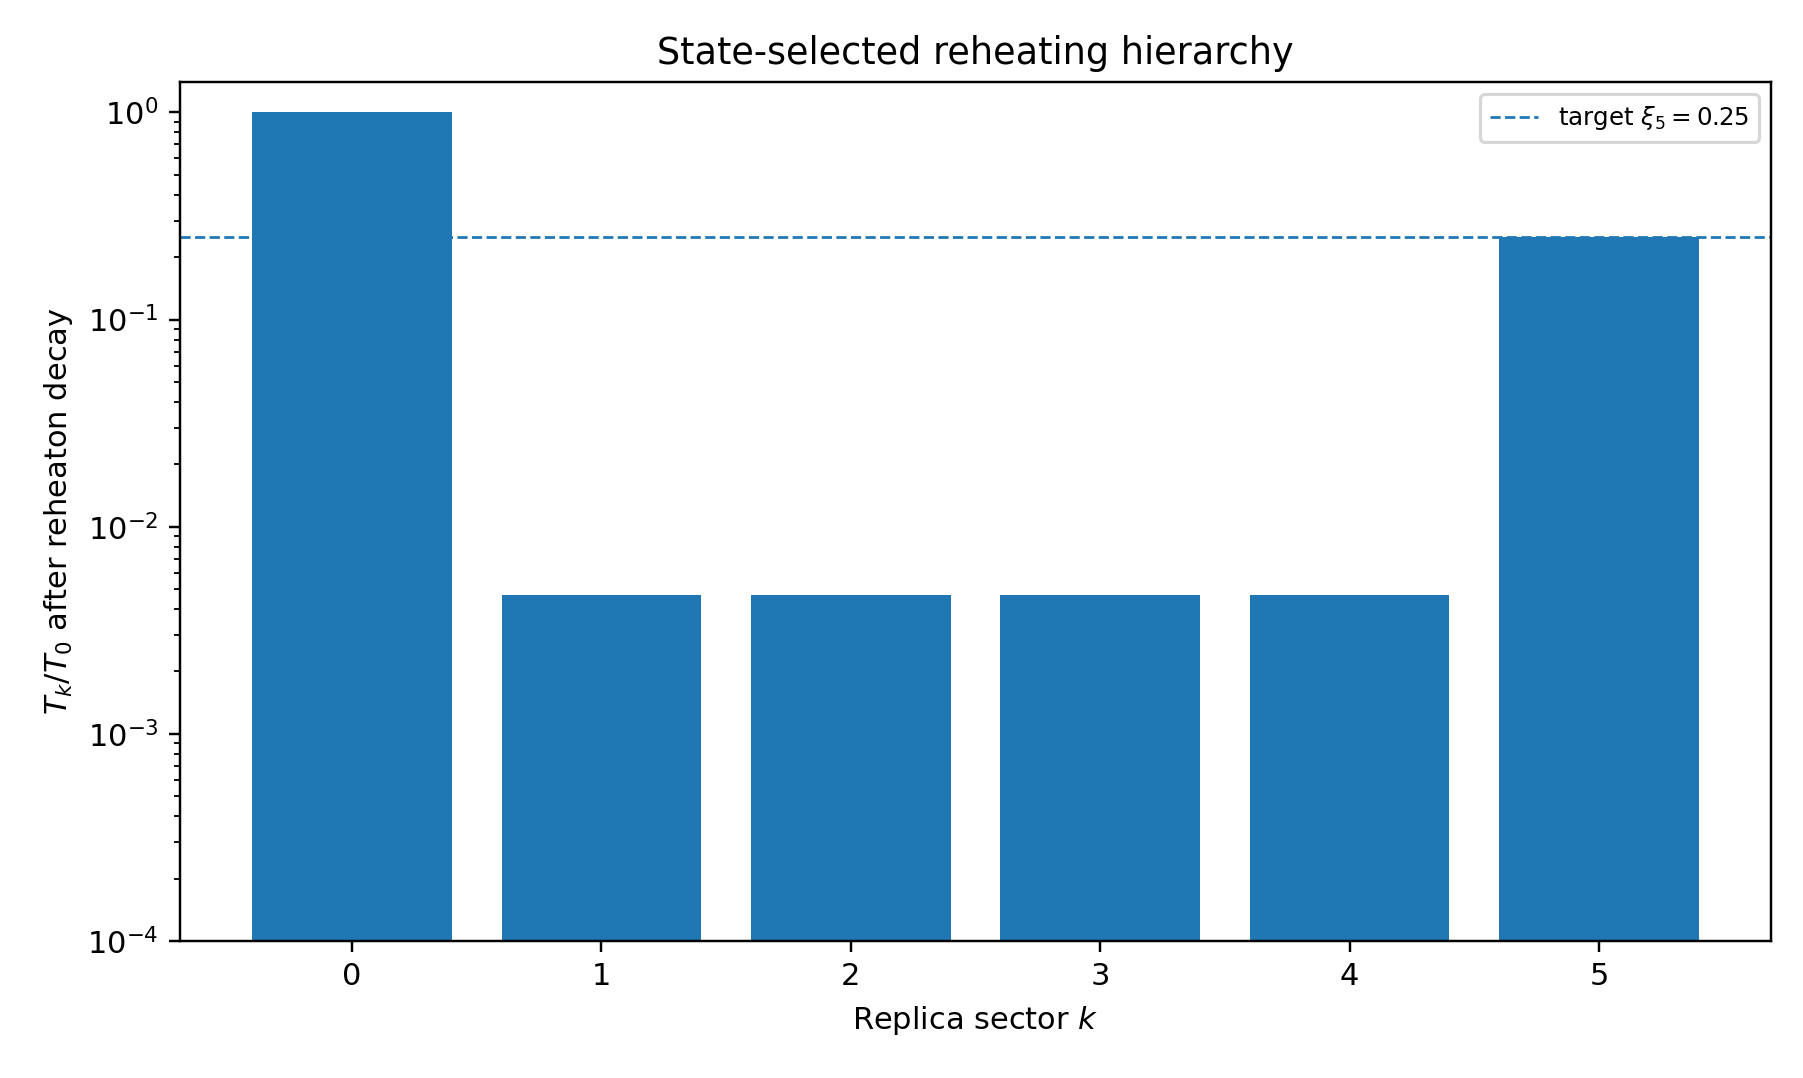
\includegraphics[width=0.92\textwidth,height=\textheight]{state_selected_sector_temperatures_v0_9.png}
\caption{The selected reheaton populates sector 0, the clockwise
adjacent sector 5, and only a gravity-level floor in the remaining
sectors.}
\end{figure}

\section{Transient one-hot selector}\label{transient-one-hot-selector}

\subsection{Selector potential}\label{selector-potential}

A hard sector label is forbidden, so the model must select \(R_0\)
dynamically. Introduce a \(Z_6\)-singlet trigger field \(D\) and the
orbit-symmetric potential

\[
\begin{aligned}
V_Q
={}&
\frac{\lambda_Q}{4}
\left[
\sum_k|Q_k|^2
-v_Q^2F(D)
\right]^2
+
\frac{\kappa_Q}{2}
\sum_{k<\ell}|Q_k|^2|Q_\ell|^2
\\
&+
\frac{m_{Q0}^2}{2}
\left[1-F(D)\right]
\sum_k|Q_k|^2.
\end{aligned}
\]

The switching function satisfies

\[
F(0)=1,
\qquad
F(v_D)=0.
\]

A concrete smooth choice is

\[
F(D)=
\frac12
\left[
1-\tanh\left(\frac{D^2-D_c^2}{\Delta_D^2}\right)
\right].
\]

While \(D\simeq0\), the positive \(\kappa_Q\) term makes the minima
one-hot:

\[
|Q_j|=v_Q,
\qquad
Q_{k\neq j}=0.
\]

There are six symmetry-related choices. Inflation selects one
homogeneous branch, which we label \(j=0\).

When \(D\) rolls to \(v_D\), the unique vacuum is

\[
Q_k=0
\qquad
\forall k.
\]

Thus the selector breaks \(Z_6\) only as a transient state and restores
the exact symmetric vacuum before the late Universe.

\subsection{Kinematic isolation}\label{kinematic-isolation}

Couple the selector to the reheaton orbit through

\[
V_{QR}
=
\frac{\lambda_{QR}}2
\sum_k
\left(X_k^2+Y_{k-1}^2\right)
\sum_{j\neq k}|Q_j|^2.
\]

This is exactly cyclic. On the branch \(Q_0=v_Q\),

\[
\Delta m_{R,0}^2=0,
\]

while every \(k\neq0\) pair receives

\[
\Delta m_{R,k}^2
=
\lambda_{QR}v_Q^2.
\]

Take

\[
v_Q=10^{10}\ {\rm GeV},
\qquad
\lambda_{QR}=0.50,
\qquad
\kappa_Q=0.25.
\]

Then

\[
m_{Q,\perp}
=
\sqrt{\kappa_Q}v_Q
=5.0\times10^9\ {\rm GeV}
=50H_*,
\]

and

\[
m_{R,k\neq0}
=
\sqrt{m_R^2+\lambda_{QR}v_Q^2}
=7.14\times10^9\ {\rm GeV}.
\]

For a post-inflation inflaton mass

\[
m_\phi=10^{10}\ {\rm GeV},
\]

only

\[
\phi\to R_0R_0
\]

is kinematically open:

\[
m_R<m_\phi/2,
\]

whereas

\[
m_S>m_\phi/2,
\qquad
m_{R,k\neq0}>m_\phi/2.
\]

\begin{figure}
\centering
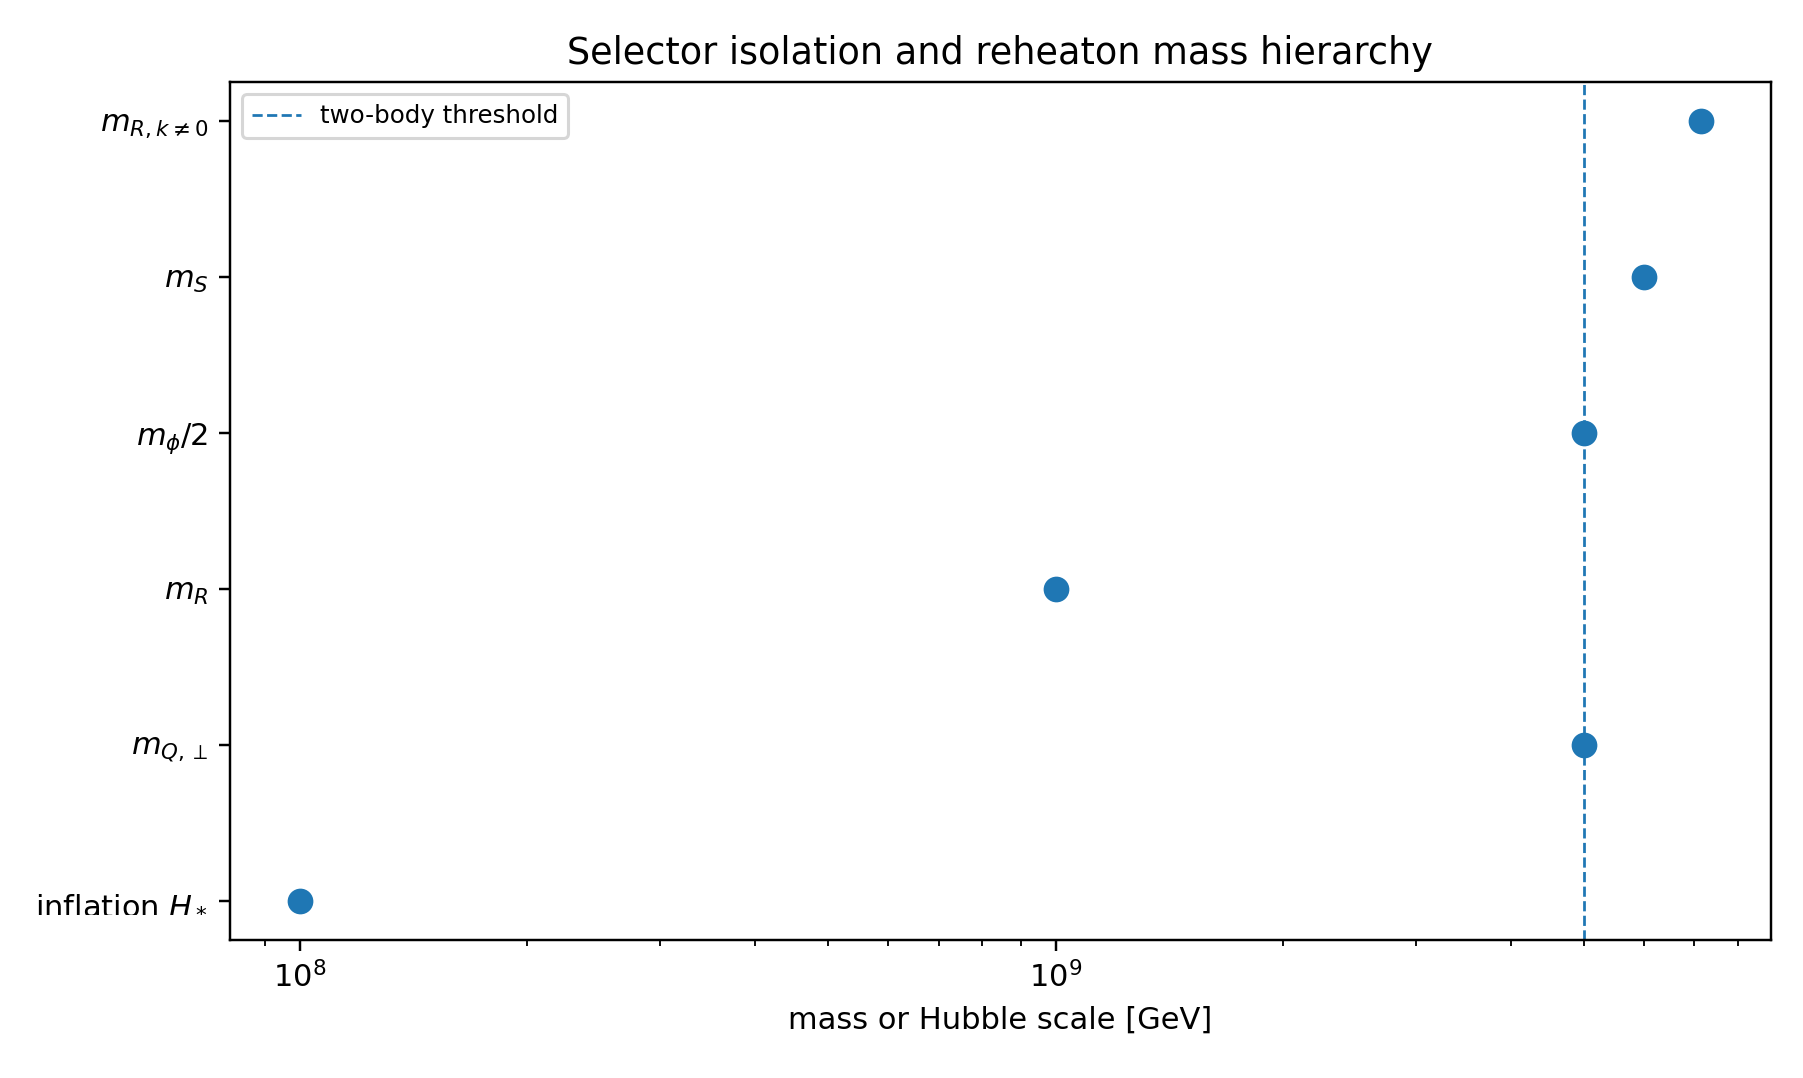
\includegraphics[width=0.92\textwidth,height=\textheight]{state_selected_mass_hierarchy_v0_9.png}
\caption{Only the selected light reheaton lies below the inflaton
two-body threshold.}
\end{figure}

\section{Cosmological chronology}\label{cosmological-chronology}

The required temporal ordering can be expressed as

\[
\boxed{
\Gamma_{\phi\to R_0R_0}
\gg
\Gamma_Q
\gg
\Gamma_R.
}
\]

An illustrative benchmark is

\[
\Gamma_\phi=100\ {\rm GeV},
\qquad
\Gamma_Q=1\ {\rm GeV},
\qquad
\Gamma_R=1.4135\times10^{-2}\ {\rm GeV}.
\]

The history is then:

\begin{enumerate}
\def\labelenumi{\arabic{enumi}.}
\tightlist
\item
  \textbf{Inflation.} The selector is in the one-hot branch \(Q_0=v_Q\).
  All observable modes leave the horizon in the same branch.
\item
  \textbf{Inflaton decay.} The inflaton coupling is democratic, \[
  \mathcal L_{\phi R}
  =
  -\frac{g_{\phi R}}2
  \phi\sum_k(X_k^2+Y_k^2),
  \] but kinematics permits only \(R_0\) production.
\item
  \textbf{Selector restoration.} After the inflaton population has
  disappeared, \(D\) rolls and all \(Q_k\) return to zero. The vacuum
  action is again manifestly \(Z_6\)-symmetric.
\item
  \textbf{Reheaton domination and decay.} The already produced \(R_0\)
  quanta do not oscillate into other replica labels because no
  off-diagonal \(k\)-mixing exists. They decay later into sectors 0 and
  5 with the fixed branching fractions above.
\item
  \textbf{Thermal focusing.} The resulting \((\xi_0,\xi_5)=(1,0.25)\)
  state generates the thermal phasor and QCD focusing used in v0.8.
\end{enumerate}

This sequence is the reason the model avoids a permanent lower-harmonic
potential. The selector background is gone before electroweak symmetry
breaking and before the vacuum spectrum is measured.

\section{Reheat scale and leakage}\label{reheat-scale-and-leakage}

The visible radiation density at reheaton decay is

\[
\rho_0
=
B_0\,3M_{\rm Pl}^2\Gamma_R^2
=
\frac{\pi^2}{30}g_*T_0^4.
\]

For

\[
g_*=106.75,
\qquad
T_0=1.002\times10^8\ {\rm GeV},
\]

this gives

\[
\boxed{
\Gamma_R=1.4135\times10^{-2}\ {\rm GeV}.
}
\]

The required trilinear scale is

\[
\boxed{
\mu_H
=
\sqrt{8\pi m_R\Gamma_R}
=1.8848\times10^4\ {\rm GeV}.
}
\]

The visible and adjacent couplings are

\[
\mu_0=1.8811\times10^4\ {\rm GeV},
\]

\[
\mu_5=1.1757\times10^3\ {\rm GeV}.
\]

A conservative gravity-mediated width into any one otherwise empty
replica is

\[
\Gamma_{\rm grav}^{(k)}
\lesssim
\frac{m_R^3}{8\pi M_{\rm Pl}^2}
=6.71\times10^{-12}\ {\rm GeV}.
\]

Therefore

\[
B_{\rm grav}^{(k)}
\lesssim4.75\times10^{-10}
\]

and

\[
\boxed{
\xi_{1,2,3,4}
\lesssim4.67\times10^{-3}.
}
\]

These sectors contribute negligibly to both the reheating phasor and
\(N_{\rm eff}\).

Integrating out \(R_0\) also generates a cross-sector Higgs quartic. A
conservative one-loop estimate is

\[
\lambda_{05}^{\rm loop}
\sim
\frac{(\mu_0\mu_5)^2}{16\pi^2m_R^4}
=3.10\times10^{-24},
\]

far below the value needed to equilibrate the sectors.

The simple Higgs portal does introduce a visible Higgs mass correction
of order

\[
\delta m_H^2
\sim
\frac{\mu_0^2}{16\pi^2}
=2.24\times10^6\ {\rm GeV}^2.
\]

This corresponds to a scale near \(1.5\) TeV. It is not catastrophic for
an EFT benchmark, but it is inelegant. A fermionic thermalizer portal,
or a cascade through a protected intermediate sector, is preferable in a
final UV model.

\section{Why radiative protection is
retained}\label{why-radiative-protection-is-retained}

The complete vacuum Lagrangian contains the six interactions

\[
X_kH_k^\dagger H_k,
\qquad
Y_kH_k^\dagger H_k,
\]

with common coefficients. It also contains the complete oriented orbit

\[
X_kY_{k-1}.
\]

No coefficient singles out \(k=0\). Hence any zero-temperature
counterterm generated in the symmetric vacuum must itself be a
\(Z_6\)-invariant orbit sum.

The temporary selector background can generate a time-dependent
one-sector correction while \(Q_0\neq0\). This is a finite-background
effect and is allowed to produce low harmonics during reheating. Indeed,
such a term strengthens vacuum focusing. But after

\[
Q_k\to0,
\]

it cannot remain as a sector-dependent renormalised parameter unless the
theory contains either:

\begin{itemize}
\tightlist
\item
  a remanent selector expectation value;
\item
  a hard \(Z_6\)-violating counterterm;
\item
  a non-decaying asymmetric condensate that couples to the coloured
  thresholds;
\item
  or an anomaly that explicitly violates the cyclic symmetry.
\end{itemize}

The first three are absent by construction. The fourth must be excluded
in a UV discrete-gauge completion.

The remaining rigorous task is a two-loop Schwinger-Keldysh calculation
with the transient \(Q_0(t)\) background. That calculation must verify
that the non-equilibrium state produces only finite-density terms that
vanish with its occupation and does not leave an unsuppressed matching
coefficient in the late vacuum EFT.

\section{Domain walls and defects}\label{domain-walls-and-defects}

\subsection{Selector walls}\label{selector-walls}

During inflation the selector potential has six one-hot minima. The
angular barrier between adjacent branches is of order

\[
\Delta V_Q
\sim
\frac{\kappa_Qv_Q^4}{8}.
\]

For the benchmark,

\[
\frac{\Delta V_Q}{H_*^4}
\sim3.1\times10^6.
\]

The non-selected selector modes also satisfy

\[
\frac{m_{Q,\perp}}{H_*}=50.
\]

Inflation therefore places the observable patch in one branch with
exponentially suppressed hopping. When the trigger restores

\[
Q_k=0,
\]

the discrete symmetry is restored to a unique vacuum. Restoration
removes walls rather than creating a new broken phase.

\subsection{Chronometric-field walls}\label{chronometric-field-walls}

The compact chronometric field has

\[
f_a=2.435\times10^{10}\ {\rm GeV},
\]

while

\[
T_R=1.002\times10^8\ {\rm GeV}.
\]

Thus

\[
\frac{T_R}{f_a}=4.12\times10^{-3}.
\]

The symmetry is assumed broken before inflation and not thermally
restored. Inflationary phase noise is

\[
\frac{H_*}{2\pi f_a}
=6.54\times10^{-4},
\]

whereas the reheating-selected thermal phase is

\[
x_T=0.05244.
\]

The bias exceeds the inflationary fluctuation by a factor of
approximately 80. A single observable branch is therefore selected.

A stronger UV option is to embed the residual discrete transformation
into a continuous gauge group, in the spirit of the Lazarides-Shafi
mechanism. Then apparently distinct vacua can be gauge equivalent. That
is not required for the pre-inflation benchmark, but it would make the
defect argument less dependent on the thermal history.

\section{Inflation model and primary
spectrum}\label{inflation-model-and-primary-spectrum}

Use a hilltop-hybrid potential

\[
\begin{aligned}
V_{\rm inf}(\phi,W)
={}&
V_0
\left[
1-\frac{c_2}{2}\frac{\phi^2}{M_{\rm Pl}^2}
+\cdots
\right]
\\
&+
\frac{\lambda_W}{4}(W^2-v_W^2)^2
+
\frac{g_W^2}{2}\phi^2W^2.
\end{aligned}
\]

For \(\phi<\phi_c\) or \(\phi>\phi_c\), depending on convention, the
waterfall field is stabilized at the origin and supplies the vacuum
energy. A critical value terminates inflation and allows the
post-inflation inflaton mass to be much larger than its slow-roll
curvature.

Take

\[
H_*=10^8\ {\rm GeV},
\qquad
A_s=2.10\times10^{-9},
\qquad
n_s=0.9682.
\]

The slow-roll parameters are

\[
\epsilon_*
=
\frac{H_*^2}{8\pi^2A_sM_{\rm Pl}^2}
=1.017\times10^{-14},
\]

\[
\eta_*
=
\frac{n_s-1+6\epsilon_*}{2}
=-0.01590.
\]

Therefore

\[
\boxed{
r=16\epsilon_*=1.63\times10^{-13}.}
\]

The inflationary energy scale is

\[
V_0^{1/4}
=
2.05\times10^{13}\ {\rm GeV}.
\]

For the local quadratic hilltop approximation,

\[
c_2=0.01590,
\]

\[
\frac{\phi_*}{M_{\rm Pl}}
=8.97\times10^{-6},
\]

and, for 55 e-folds,

\[
\frac{\phi_c}{M_{\rm Pl}}
=2.15\times10^{-5}.
\]

The single-clock consistency estimate is

\[
\boxed{
f_{\rm NL}^{\rm local}
\simeq
\frac5{12}(1-n_s)
=0.0133.}
\]

This inflationary block is phenomenologically adequate but not yet a
complete UV model. Low-scale hybrid inflation is notoriously sensitive
to radiative and higher-dimensional corrections; a shift-symmetric,
supersymmetric or four-form completion is required for a
first-principles construction.

\section{Curvature transfer through reheaton
decay}\label{curvature-transfer-through-reheaton-decay}

Suppose \(R_0\) dominates before it decays. On the decay hypersurface,

\[
\rho_i=B_i\rho_R.
\]

For radiation,

\[
\zeta_i
=
-\psi
+
\frac14\frac{\delta\rho_i}{\rho_i}.
\]

Therefore

\[
\boxed{
\zeta_i
=
\zeta_R
+
\frac14\delta\ln B_i.
}
\]

The relative entropy perturbation is

\[
S_{50}
=3(\zeta_5-\zeta_0)
=
\frac34
\delta\ln\frac{B_5}{B_0}.
\]

In the present model the branching fractions are constants fixed by a
heavy mass matrix. Hence

\[
\delta B_0=\delta B_5=0
\]

and

\[
\boxed{S_{50}=0.}
\]

If the mixing angle were controlled by a fluctuating light modulus, then

\[
\delta\ln\frac{B_5}{B_0}
=
\delta\ln\tan^2\theta
=
\frac{2\delta\theta}{\sin\theta\cos\theta},
\]

so

\[
S_{50}
=
\frac{3\delta\theta}{2\sin\theta\cos\theta}.
\]

At \(\tan\theta=1/16\), this would strongly amplify \(\delta\theta\).
The mixing angle must therefore be a genuine heavy-sector parameter, not
a light modulating field. The benchmark satisfies this: \(m_R/H_*=10\),
\(m_S/H_*=60\), and the selector angular modes have \(m/H_*=50\).

\section{Chronometric spectator
perturbations}\label{chronometric-spectator-perturbations}

The superhorizon perturbation of

\[
x=a/f_a
\]

obeys

\[
\delta x''
+
\left(3+\frac{d\ln H}{d\ln a}\right)\delta x'
+
\frac{V_{,xx}(x,t)}{f_a^2H^2}\delta x
=0,
\]

where primes denote derivatives with respect to \(\ln a\). The effective
curvature includes:

\begin{itemize}
\tightlist
\item
  the protected zero-temperature \(Z_6\) potential;
\item
  the visible and adjacent heavy-threshold thermal free energies;
\item
  the visible and adjacent QCD trace anomalies;
\item
  homogeneous baryon locking.
\end{itemize}

Using the strong-attractor v0.8 benchmark,

\[
N=6,
\quad
M=1.002\times10^6\ {\rm GeV},
\quad
f_a=2.435\times10^{10}\ {\rm GeV},
\]

\[
\epsilon=2.70\times10^{-13},
\quad
m_a=7.5\times10^{-29}\ {\rm eV},
\quad
d_g=10^{-6},
\]

and the reheating temperatures derived above, the inflationary
fluctuation is

\[
\delta x_{\rm reh}
=
6.536\times10^{-4}.
\]

The numerical transfer at recombination is

\[
\boxed{
T_x^{\rm rec}
\equiv
\left|\frac{\delta x_{\rm rec}}{\delta x_{\rm reh}}\right|
=1.013\times10^{-6}.
}
\]

Hence

\[
\delta x_{\rm rec}
=-6.62\times10^{-10}.
\]

The QCD-lock perturbation is

\[
\delta\ln\frac{\Lambda_3}{\chi}
\simeq
\frac{2}{27}\epsilon\,\delta x,
\]

so

\[
\boxed{
\left|\delta\ln\frac{\Lambda_3}{\chi}\right|_{\rm rec}
=1.32\times10^{-23}.
}
\]

The field undergoes a late tachyonic release after recombination. At the
numerical endpoint \(z=71.1\),

\[
\left|\frac{\delta x}{\delta x_{\rm reh}}\right|
=3.57\times10^{-3},
\]

but even there

\[
\left|\delta\ln\frac{\Lambda_3}{\chi}\right|
=4.67\times10^{-20}.
\]

The field energy fraction is already negligible, so this late growth
does not generate an observable isocurvature component.

\begin{figure}
\centering
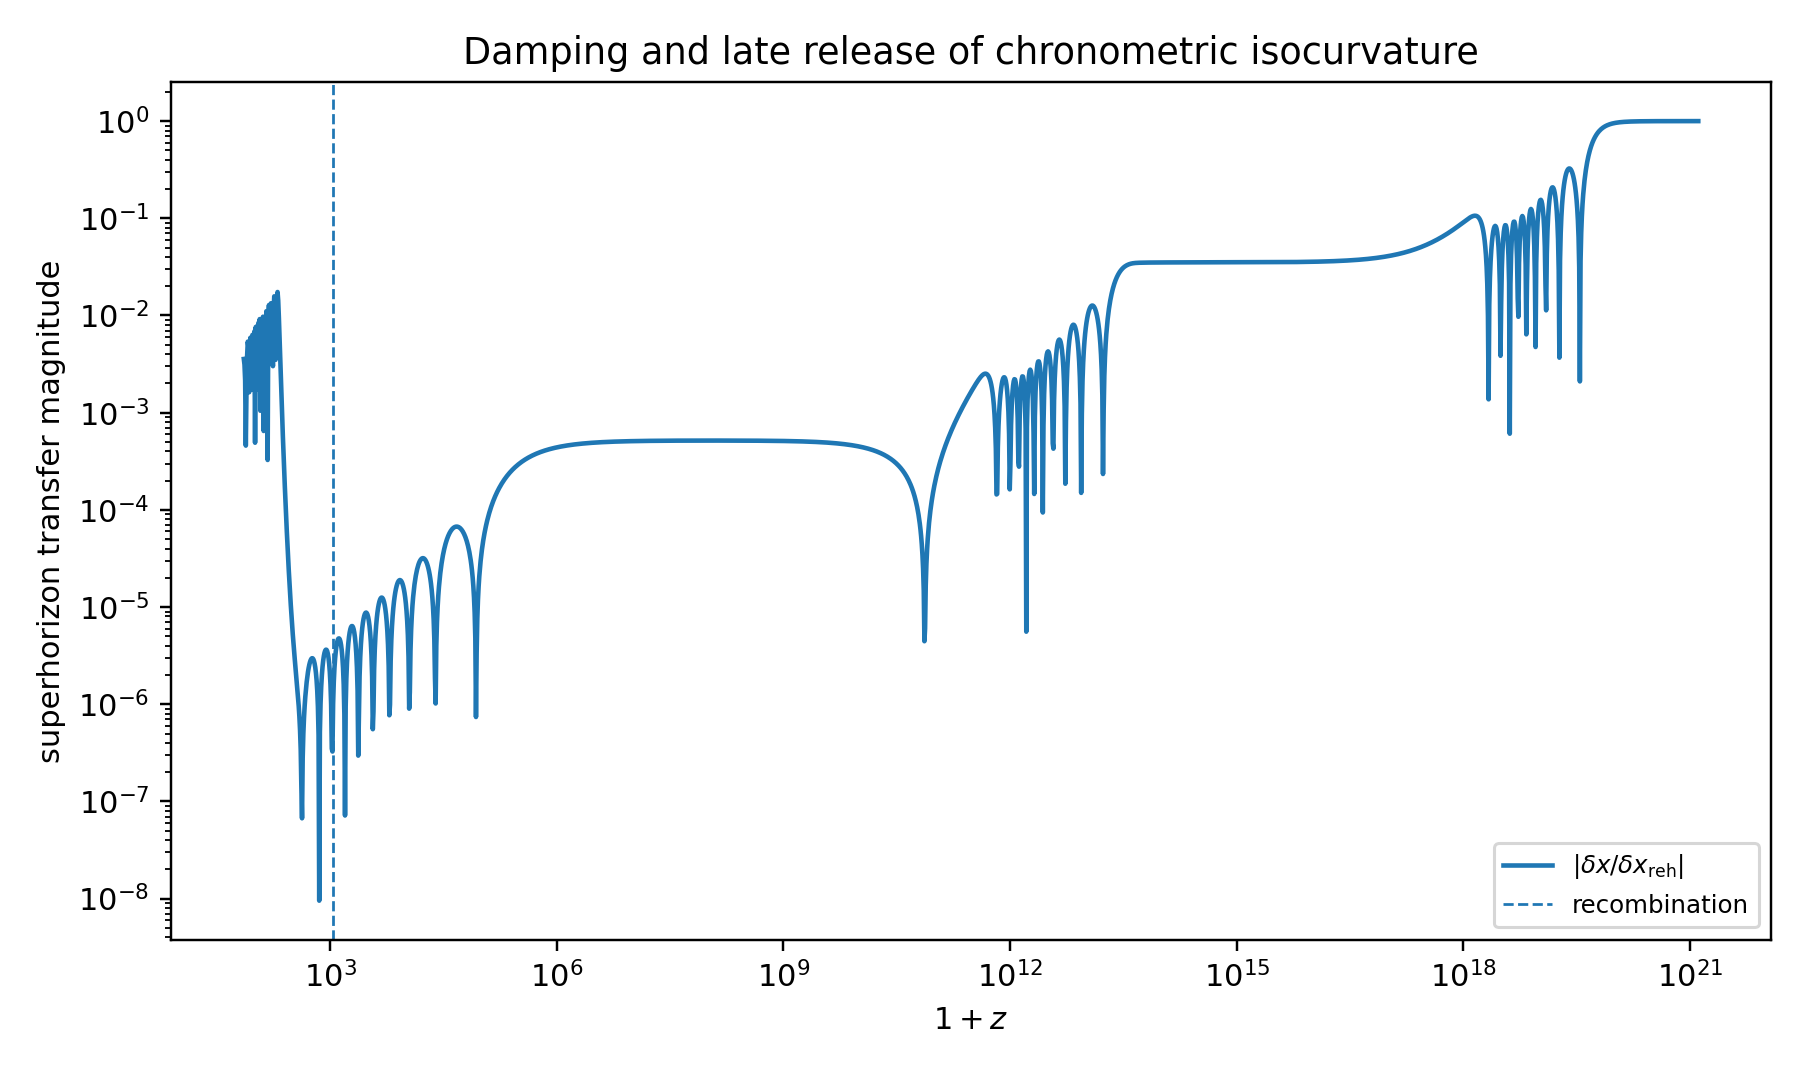
\includegraphics[width=0.92\textwidth,height=\textheight]{state_selected_chronometric_transfer_v0_9.png}
\caption{Thermal and QCD focusing erase most of the primordial
chronometric perturbation before recombination.}
\end{figure}

\section{Primordial spectrum summary}\label{primordial-spectrum-summary}

At the pivot scale,

\[
\mathcal P_\zeta(k)
=A_s\left(\frac{k}{k_*}\right)^{n_s-1}.
\]

The linear radiation isocurvature power is

\[
\boxed{\mathcal P_{S_{50}}=0}
\]

in the exact fixed-branching approximation.

The initial power in the QCD-lock fluctuation is

\[
\mathcal P_{\delta\ln(\Lambda_3/\chi)}
=
\left[
\frac{2}{27}\epsilon
\frac{H_*}{2\pi f_a}
\right]^2
\simeq1.71\times10^{-34}.
\]

By recombination it is further reduced by

\[
(T_x^{\rm rec})^2
\simeq1.03\times10^{-12}.
\]

Thus

\[
\boxed{
\mathcal P_{\delta\ln(\Lambda_3/\chi)}^{\rm rec}
\sim1.8\times10^{-46}.
}
\]

\begin{figure}
\centering
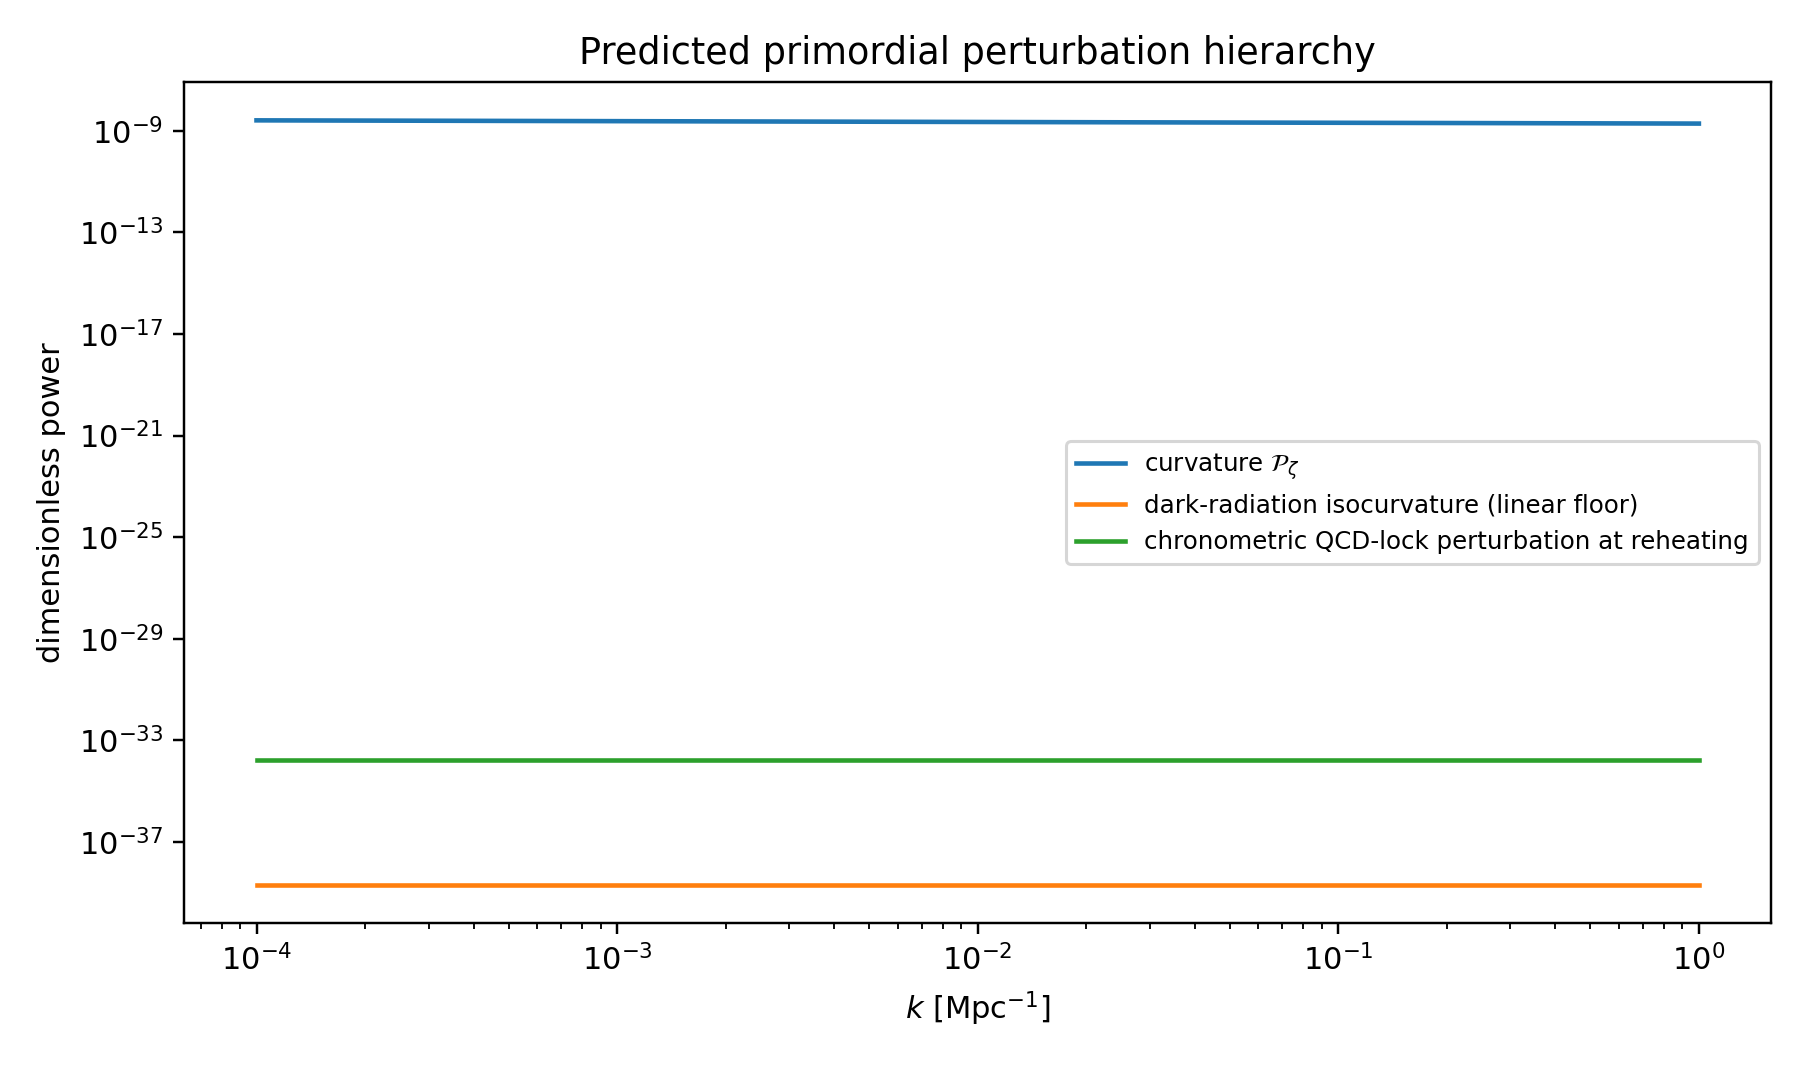
\includegraphics[width=0.92\textwidth,height=\textheight]{state_selected_perturbation_spectra_v0_9.png}
\caption{The model predicts an ordinary adiabatic curvature spectrum,
vanishing linear dark-radiation isocurvature, and a minute
chronometric-lock perturbation.}
\end{figure}

\section{Dark radiation and hidden-sector
relics}\label{dark-radiation-and-hidden-sector-relics}

For one complete adjacent Standard Model copy at \(\xi_5=0.25\), the
standard internal neutrino-photon entropy history gives approximately

\[
\Delta N_{\rm eff}
=7.403\xi_5^4
=0.0289.
\]

This is below the present 95\% bound

\[
\Delta N_{\rm eff}<0.107.
\]

The signal is potentially interesting for future CMB measurements, but
it is not accompanied by a linear dark-radiation isocurvature mode.

A full hidden-sector cosmology still requires decisions about:

\begin{itemize}
\tightlist
\item
  hidden baryogenesis;
\item
  stable hidden charged relics;
\item
  hidden neutrino masses;
\item
  hidden recombination;
\item
  whether the adjacent copy is a complete Standard Model or only the
  degrees of freedom required by cyclic protection.
\end{itemize}

The cleanest benchmark assumes no appreciable hidden baryon asymmetry
and efficient annihilation of symmetric massive relics. These
assumptions must be tested in a dedicated Boltzmann calculation.

\section{Acceptance tests}\label{acceptance-tests}

\begin{longtable}[]{@{}
  >{\raggedright\arraybackslash}p{(\columnwidth - 4\tabcolsep) * \real{0.3333}}
  >{\raggedright\arraybackslash}p{(\columnwidth - 4\tabcolsep) * \real{0.3333}}
  >{\raggedright\arraybackslash}p{(\columnwidth - 4\tabcolsep) * \real{0.3333}}@{}}
\toprule\noalign{}
\begin{minipage}[b]{\linewidth}\raggedright
Test
\end{minipage} & \begin{minipage}[b]{\linewidth}\raggedright
Result
\end{minipage} & \begin{minipage}[b]{\linewidth}\raggedright
Reason
\end{minipage} \\
\midrule\noalign{}
\endhead
\bottomrule\noalign{}
\endlastfoot
Exact cyclic action & \textbf{PASS} & All displayed couplings are
complete orbit tensors. \\
Reheaton scalar spectrum & \textbf{PASS} & Both eigenvalues are
positive; 50,000-point scan passed. \\
\(B_5/B_0=1/256\) & \textbf{PASS exactly} & Follows from
\(\tan\theta=1/16\). \\
\(\xi_5=0.25\) & \textbf{PASS exactly} & Fourth root of the energy
ratio. \\
Empty sectors & \textbf{PASS perturbatively} & No tree channel; gravity
floor \(\xi<0.005\). \\
\(\Delta N_{\rm eff}\) & \textbf{PASS} & \(0.0289<0.107\). \\
Hard reheating spurion & \textbf{ABSENT} & Asymmetry is carried by a
transient state. \\
Late vacuum radiative protection & \textbf{PASS conditionally} &
Requires no non-equilibrium remanent matching coefficient. \\
Selector isocurvature & \textbf{PASS benchmark} &
\(m_{Q,\perp}/H_*=50\). \\
Reheaton isocurvature & \textbf{PASS benchmark} & \(m_R/H_*=10\). \\
Radiation isocurvature & \textbf{ZERO at linear order} & One parent,
fixed branchings. \\
Chronometric isocurvature & \textbf{PASS} & QCD-lock fluctuation
\(<10^{-23}\) at recombination. \\
Selector domain walls & \textbf{PASS conditionally} & Inflation selects
one branch; later restoration gives unique origin. \\
Chronometric walls & \textbf{PASS conditionally} & Pre-inflation
breaking and no thermal restoration. \\
Nonperturbative reheaton production & \textbf{OPEN} & Requires lattice
preheating. \\
Exact discrete symmetry in quantum gravity & \textbf{OPEN} & Requires a
discrete-gauge embedding. \\
Full CMB likelihood & \textbf{OPEN} & Requires CLASS/CAMB
implementation. \\
\end{longtable}

\section{Novelty boundary}\label{novelty-boundary}

The following ingredients are established separately:

\begin{itemize}
\tightlist
\item
  asymmetric reheating in theories with exact or approximately exact
  exchange symmetries;
\item
  kinematic reheating asymmetry;
\item
  inflationary selection of one symmetry-related branch;
\item
  cyclic replicated sectors protecting a compact scalar potential;
\item
  fixed-branching adiabatic decay;
\item
  attractor suppression of spectator isocurvature;
\item
  inflation or gauged discrete symmetries as remedies for domain walls.
\end{itemize}

The generic radiative objection to sector-specific reheating is also
established: a hard selector coupling acts as a permanent spurion and
spoils the cyclic cancellation.

The candidate contribution is the restricted conjunction

\[
\boxed{
\begin{gathered}
\text{exact }Z_6\text{ vacuum action}
+
\text{transient one-hot state selection}
+
\text{chiral two-orbit reheaton}
\\
+
\xi_5=1/4
+
\text{zero linear dark-radiation isocurvature}
+
\text{numerically erased chronometric isocurvature}
\\
+
\text{the visible }2/27\text{ QCD chronometric response}.
\end{gathered}
}
\]

A targeted search found no exact indexed match for that full
construction. This is a plausible novelty claim, not yet a secure
priority claim. Backward and forward citation chaining, INSPIRE/ADS
searches and specialist review are still required.

\section{Next decisive calculations}\label{next-decisive-calculations}

The remaining work is sharply defined.

\subsection{Non-equilibrium radiative
matching}\label{non-equilibrium-radiative-matching}

Compute the two-loop in-in effective action in the transient background

\[
Q_0(t)\neq0,
\qquad
Q_{k\neq0}=0,
\]

and prove that all lower-harmonic terms vanish as

\[
Q_0(t)\to0
\]

and the reheaton occupation dilutes. This is the hard
radiative-stability test.

\subsection{Lattice preheating}\label{lattice-preheating}

Simulate the waterfall, selector and reheaton fields to verify that:

\begin{itemize}
\tightlist
\item
  \(R_0\) is produced efficiently;
\item
  \(R_{k\neq0}\) and \(S_k\) are not resonantly excited;
\item
  selector restoration does not create persistent walls;
\item
  nonlinear fluctuations do not modulate \(B_5/B_0\).
\end{itemize}

\subsection{Full perturbation
transfer}\label{full-perturbation-transfer}

Implement the model in a Boltzmann code with:

\begin{itemize}
\tightlist
\item
  adiabatic hidden radiation;
\item
  \(\Delta N_{\rm eff}=0.0289\);
\item
  the late chronometric-field release;
\item
  hidden-sector recombination and free streaming;
\item
  metric sources in the \(\delta x\) equation.
\end{itemize}

The leading analytic prediction is already clear:

\[
S_{50}=0,
\qquad
r\simeq1.6\times10^{-13},
\qquad
\delta\ln(\Lambda_3/\chi)_{\rm rec}\sim10^{-23}.
\]

\subsection{UV completion}\label{uv-completion}

Replace the global cyclic symmetry by an anomaly-free discrete gauge
symmetry or a continuous gauge group whose remnant is \(Z_6\). The UV
model must preserve the oriented nearest-neighbour coupling while
forbidding all hard lower-harmonic operators.

\section{Final assessment}\label{final-assessment}

The requested reheating pattern is achievable without surrendering the
protected cyclic action.

The successful architecture is not

\[
\text{one reheaton with an explicitly privileged sector}.
\]

It is

\[
\boxed{
\text{a complete }Z_6\text{ reheaton orbit}
+
\text{a transient inflation-selected state}
+
\text{fixed chiral neighbour mixing}.
}
\]

That construction gives

\[
(\xi_0,\xi_1,\xi_2,\xi_3,\xi_4,\xi_5)
\simeq
(1,<0.005,<0.005,<0.005,<0.005,0.25),
\]

while preserving the late-time vacuum symmetry.

Its most important perturbative prediction is not an exotic isocurvature
spectrum, but its absence:

\[
\boxed{
\text{one parent plus fixed branching ratios produces adiabatic visible and hidden radiation.}
}
\]

The chronometric field's own inflationary fluctuations are then erased
by the same thermal and QCD dynamics that select its vacuum. The
resulting cosmology is unusually clean:

\[
\boxed{
\text{nonzero homogeneous chronometric shear}
\quad+
\text{essentially standard adiabatic primordial perturbations}.
}
\]

The model now fails or succeeds on two concrete calculations:
non-equilibrium radiative matching and lattice reheating. The former
tests whether the state/action distinction truly protects the vacuum;
the latter tests whether the elegant branching algebra survives violent
nonlinear dynamics.

\section{References}\label{references}

\begin{enumerate}
\def\labelenumi{\arabic{enumi}.}
\tightlist
\item
  C. Delaunay et al., \emph{Natural Phantom Crossing from Axion-WIMP
  Interactions}, arXiv:2607.28721. Appendix A derives the generic
  hard-spurion obstruction to asymmetric reheating in a cyclic
  replicated theory.
\item
  N. Craig, S. Koren and T. Trott, \emph{Cosmological Signals of a
  Mirror Twin Higgs}, arXiv:1611.07977. Develops asymmetric reheating
  while respecting an exact, spontaneously broken exchange symmetry.
\item
  L. Balkenhol et al., \emph{Inflation at the End of 2025: Constraints
  on r and n\_s Using the Latest CMB and BAO Data}, arXiv:2512.10613.
\item
  \emph{A 2\% Determination of N\_eff from Primordial Element Abundance,
  Cosmic Microwave Background, and Baryon Acoustic Oscillation
  Measurements}, arXiv:2603.13226.
\item
  G. K. Karananas and M. Shaposhnikov, \emph{A Scaling Non-Compact QCD
  Axion}, arXiv:2606.17019. Provides a recent example of dynamical
  post-inflationary isocurvature erasure.
\item
  B. A. Bassett, S. Tsujikawa and D. Wands, \emph{Inflation Dynamics and
  Reheating}, arXiv:astro-ph/0507632.
\item
  C. P. Burgess et al., \emph{Revisiting Two-Field Hybrid Inflation as
  an Effective Field Theory}, arXiv:2006.13960.
\item
  C. Coriano et al., \emph{Gauging Axionic Symmetries and Dark Matter},
  arXiv:2604.25888. Reviews the Lazarides-Shafi domain-wall mechanism.
\item
  The preceding project notes v0.5-v0.8 for the all-orders QCD threshold
  lock, the \(2/27\) transmission coefficient, cyclic radiative
  protection, environmental non-screening and cosmological vacuum
  selection.
\end{enumerate}

\end{document}
